\section{Arrivé sur Bali}

Date: 07/04/2008

\begin{multicols}{2}

Salut tout le monde !!! Bon alors, autant vous le dire tout de suite, vu les photos qui sont dans cet article, vous allez me détester quand vous les aurez vues... enfin disons qu'il y a de fortes chances... Arrivé mercredi, sans aucun souci durant le trajet, Patrick est venu me chercher à l'aéroport pour aller au bateau, joli canot de 13m50, bien équipé pour la navigation, spacieux. Nous sommes allés faire un petit tour à Kuta, coin le plus touristique de Bali, Plage très appréciée des surfers du monde entier. En fait j'ai adoré le passage ombragé qui longe la route et la plage, où une multitude des petits vendeurs proposent location de planche de surf, boissons fraîches et massages, vraiment très tentant.

\hspace*{-0.65cm}
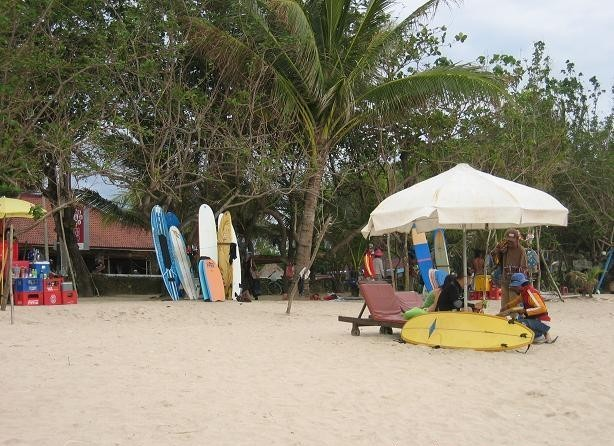
\includegraphics[width=4.8cm]{articles/Arrivee-sur-bali/1207567562ikVd.jpg}
Plage de Kuta

Sylvie, une amie de Patrick, est arrivée avec sa fille Tamara le soir, pendant que j'étais dans les bras de Morphée, décalage horaire oblige. Nous somme partis jeudi et revenus samedi matin pour faire un tour dans Bali, en s'arrêtant dans des petits hôtels bien sympathiques (c'est un euphémisme) avec vue sur mer, cocotiers, piscines, eau à 30 degrés quand elle est froide...

\hspace*{-0.65cm}
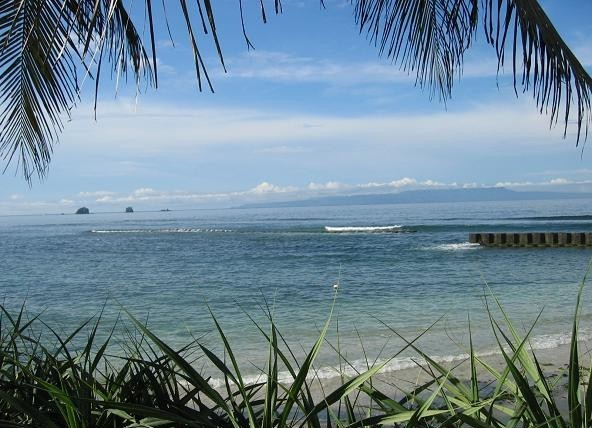
\includegraphics[width=4.8cm]{articles/Arrivee-sur-bali/1207567561DqJk.jpg}
La mer

\hspace*{-0.65cm}
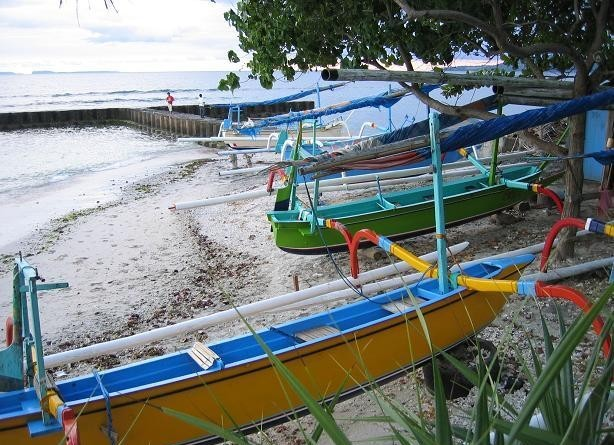
\includegraphics[width=4.8cm]{articles/Arrivee-sur-bali/1207567564x5vI.jpg}
Bateau de pêche traditionnels

\hspace*{-0.65cm}
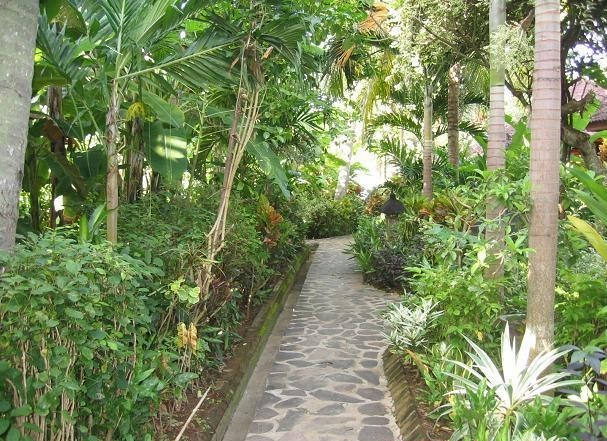
\includegraphics[width=4.8cm]{articles/Arrivee-sur-bali/120756756426sq.jpg}
L'allée d'un hôtel

\hspace*{-0.65cm}
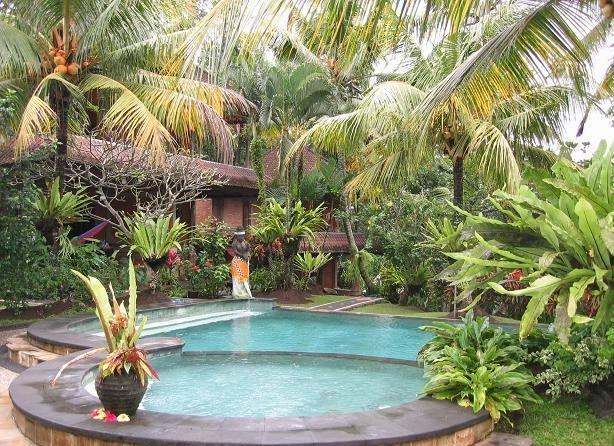
\includegraphics[width=4.8cm]{articles/Arrivee-sur-bali/1207567563njCA.jpg}
Ze piscine

La capitale de l'île est Denpasar, ville qui grouille de partout, sans gros interêt à ce que l'on m'a dit, j'irais voir quand même... L'aéroport est à Kuta, juste au Sud de Denpasar, ville beaucoup plus jolie... et touristique. En ce qui me concerne, le bateau est à la Marina de Benoa, juste à l'Est de Kuta. Je connaissais deja un peu l'artisanat de Bali, les balinais font de magnifiques objets de déco, des tissus, des sculptures, on en voit partout. Ici une photo prise au bord de la route dans un petit village

\hspace*{-0.65cm}
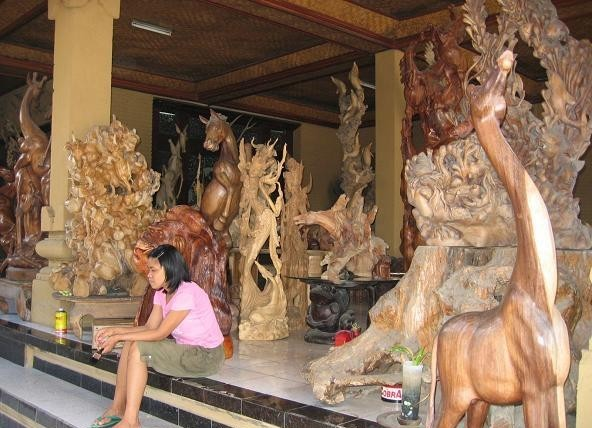
\includegraphics[width=4.8cm]{articles/Arrivee-sur-bali/1207567562ISpn.jpg}
Sculptures en bois

Dans les jours qui suivent je vais louer un scooter pour faire un tour complet de l'île, essayer d'aller voir un pote de Patrick, Indonésien, plus au Nord dans l'île, monter sur le plus gros volcan, me perdre dans les rizières, enfin pas trop de plans a l'avance, il est très facile de se loger ici, les gens sont aussi sympa qu'en Inde, et bizarrement l'immense majorité des personnes que l'on voit ont entre 20 et 25 ans.

A bientôt.

\end{multicols}
